

\definecolor{darkgreen}{rgb}{0.2,0.6,0.2}
\lstdefinelanguage{JavaScript}{
  keywords={typeof, new, true, false, catch, function, return, null, catch, switch, var, if, in, while, do, else, case, break},
  keywordstyle=\color{blue}\bfseries,
  ndkeywords={class, export, boolean, throw, implements, import, this},
  ndkeywordstyle=\color{darkgray}\bfseries,
  identifierstyle=\color{black}\bfseries,
  sensitive=false,
  comment=[l]{//},
  morecomment=[s]{/*}{*/},
  commentstyle=\color{purple}\ttfamily,
  stringstyle=\color{darkgreen}\ttfamily,
  morestring=[b]',
  morestring=[b]"
}

\lstset{
   language=JavaScript,
   backgroundcolor=\color{lightgray},
   extendedchars=true,
   basicstyle=\footnotesize\ttfamily\bfseries,
   showstringspaces=false,
   showspaces=false,
   %numbers=left,
   %numberstyle=\footnotesize,
   %numbersep=9pt,
   tabsize=2,
   breaklines=true,
   showtabs=false,
   captionpos=b,
   aboveskip=9pt,
   belowskip=9pt,
}

%----------------------------------------------------------------------------
\chapter{Technológiai áttekintés}
%----------------------------------------------------------------------------
A következő alfejezetekben a felhasznált technológiákra fogok kitérni több hangsúlyt fektetve azokra a technológiákra amik vagy újabbak vagy fontosabb szerepet játszottak az elkészült alkalmazásban.

%----------------------------------------------------------------------------
\section{Javascript}
%----------------------------------------------------------------------------

A Javascript nyelvet az útóbbi évek fejleményei miatt választottam, hiszen már lehetséges vele egy teljes kliens és szerveroldalt átívelő alkalmazást létrehozni. Szkriptnyelv jellege miatt arra számítottam, hogy gyors prototípizálásra lesz lehetőség, ez azért fontos, mert a technológiák nagy része amivel a munkámban foglalkoztam új volt számomra.

A Javascript nyelv nem kerül részletes bemutatásra, helyette arra tértem ki, ami nehezen érthető volt számomra: az , hogy hogyan tud objektumorientált lenni a nyelv, ha tud egyáltalán. 

\subsection{Prototípus öröklés a Javascriptben}

Javascript egy prototípus alapú objektumorientált nyelv, ez azt jelenti, hogy objektumok vannak, amik nem osztálypéldányok és az öröklés szempontjából minden objektumnak van egy referenciája a prototípusára, és ez addig megy tovább amíg a prototípus null lesz\cite{mdnprotoref}. 

Örökölt attribútumok esetében úgy működik a feloldás, hogy először az objektum saját attribútumai között keressük, ha nem találjuk, akkor a prototípus láncon tovább megyünk és ott keressük, és így tovább a végéig, ahol, ha nem találjuk meg akkor \lstinline{undefined} az eredmény. A függvények attribúmként viselkednek ebből a szempontból és ezáltal a függvény felüldefineálás is működik.

\subsubsection{Objektumpéldányosítás}

Több módon történik az objektumok példányosítása, az egyszerű esetekben a következőképpen néz ki a prototípus lánc: 
\begin{enumerate}
\item \lstinline| var o = { a: 1 };| esetében o az Object-ből örököl és a prototípuslánc:

 \lstinline|o ---> Object.prototype ---> null|
\item \lstinline| var a = ["egy", "meggy", "citrom"]; | esetében az \lstinline{a} egy tömb aminek a prototípusa az Object \lstinline|a ---> Array.prototype ---> Object.prototype ---> null|
\item \lstinline| function foo(){ return 0; }| a függvény is egy ``egyszerű'' objektum: 

\lstinline| foo ---> Function.prototype ---> Object.prototype ---> null| 

\item 
\begin{lstlisting}
{
    function Alma() {
        this.color = "green";
    }
    Alma.prototype = {
        ripe: function() {
            this.color = "red";
        } 
    }
    var a = new Alma();
}
\end{lstlisting}

A konstruktor az egy egyszerű function ami meghívódik a \lstinline{new} kulcsszó használatakor, ekkor a prototípuslánc: 

\lstinline| a ---> Alma.prototype ---> Object.prototype ---> null|

\end{enumerate}

Meg kell jegyezni, hogy a hosszú prototípusláncok teljesítménycsökkentést jelentenek, hiszen végig kell menni mindig a láncon egyes attribútumokért. Az is fontos, hogy a Javascript környezet annyira megengedő, hogy beépített objektumokat lehet változtatni, úgynevezett ``monkey patching''-gel, ez viszont nem javasolt, mert nehéz debuggolni, megnehezíti annak a fejlesztőnek a munkáját aki nem tud a patch-ről és ha két modul ugyanazt a kódot patch-eli, akkor amelyik később lefut az ``nyer''.



\subsection{Coffeescript}

Napjainkban nagyon sok olyan nyelv van ami Javascriptre fordul\cite{coffeeref}. A szakdolgozatom elején CoffeeScript-ben fejlesztettem a prototípust, mert egy olyan nyelv ami Javascriptre fordul, de Python jellegű szintaxisa van. A főbb jellegzetességei a következők\cite{maccaw2011}:

\begin{itemize}
\item zárójelek helyett indentálással történik a kód blokkok elválasztása, emiatt olvashatóbb lehet a kód,
\item eltávolítja a globális referencia fogalmát és csak lokális változókat lehet deklarálni,
\item nagyon rövid a függvénydeklaráció: \lstinline|function() { do() ;}| helyett \lstinline{() -> do},
\item nagyon rugalmas ciklusok és lista generálások: \lstinline{[ apple for apple in apples when not apple.rotten ]} ez egy friss alma listával tér vissza egy sorban, 
\item a feltételes blokkok és ciklusok zárójelmentesek és egyszerűbb helyes kódot írni: \begin{lstlisting}
    for i in items
        if i>5 then print i
        \end{lstlisting}
\item nagyon hasznos a feltételes tagváltozóhozzáférés: a \lstinline{apple.tree?.cutDown} kód akkor is sikeresen lefut, ha az \lstinline{apple} objektumnak nincs \lstinline{tree} tagváltozója,
\item bevezeti a Pythonhoz hasonló osztálydeklaráció szintaxist, ami félrevezető lehet, ha nem ismerjük jól a Javascriptet, hiszen csak ezen az absztrakt szinten objektumorientált, a lefordult Javascriptben prototípus öröklés lesz,
\item teljesen ekvivalens Javascript kód fordul belőle és visszafordítás is ugyanúgy lehetséges.
\end{itemize}

Igaz, hogy könnyebb üzleti logikát és funkcionális programozási kihívásokat megoldani a Coffeescript szintaxissal, de azt tapasztaltam, hogy a munkám során nem segített a keretrendszerek (AngularJS, NodeJS) megértésében, nehezebb volt a hibákat debuggolni. Amikor már ismerős volt a technológia, akkor hatékonyabb tudtam lenni Coffeescipt segítségével, de ez csak a végére alakult ki. Egy másik ok az, hogy a jelen dokumentumban sok kódrészlet szerepel és ennek megértését hátráltatja a Coffeescript szintaxis azon olvasó számára aki nem ismeri a nyelvet. 

Bármikor át lehet térni Coffeescriptre hiszen mindkét irányba lehet fordítani, tehát egy létező Javascript projektet Coffeescriptre lehet fordítani, be kell állítani az automatikus fordítást Javascriptre és már dolgozhatunk is tovább Coffeescriptben.


%----------------------------------------------------------------------------
\section{Socket.IO}
%----------------------------------------------------------------------------
A Socket.IO egy JavaScript könyvtár ami valósidejű alkalmazások kétirányú kommunikációját támogatja. Ha a hagyományos kliens-szerver weboldal modellre gondolunk, akkor azt a hiányosságot oldja meg, hogy miután letöltődik a honlap a böngészőben, nem egyértelmű, hogy hogyan tudnánk a kliens oldalon reagálni szerver oldali eseményekre. A WebSocket protokoll egy TCP kapcsolaton full-duplex kommunikációt biztosít.

Valósidejű alkalmazásra egy naív próbálkozás az egyszerű AJAX polling, ami így nézhet ki:
\medskip
\begin{lstlisting}[caption=Egyszerű polling]
setInterval(function(){
    $.ajax({ url: "server", success: function(data){
        //
    }, dataType: "json"});
}, 30000);
\end{lstlisting}

Ez több próblémát is felvet, többek között azt, hogy, ha a polling intervallum túl kicsi, akkor túl sok lekérés megy a szerverhez, ha az intervallum túl nagy, akkor nem kapunk elég gyakran értesítést. Minden egyes lekérdezés egy-egy kapcsolatfelépítést jelentene, ami pazarló lehet.

Erre egy alternatíva a Long Polling, ekkor a válasz nem érkezik meg a szervertől addig, amíg nincsen olyan esemény amiről a klienst értesítenénk:

\begin{lstlisting}[caption=Long Polling]
(function poll(){
    $.ajax({ url: "server", success: function(data){
        // 
    }, dataType: "json", complete: poll, timeout: 30000 });
})();
\end{lstlisting}

Itt is láthatunk néhány hiányosságot: újra kell kapcsolódni periodikusan, mert a kérés lejárhat (timeout) és a kommunikációs protokoll még mindig HTTP, ami overhead-et jelent.


A pollingnál egyszerűbb megoldás egy egyetlen TCP kapcsolatot kialakítani a kétirányú kommunikációra, ezt kínálja a Websocket protokoll \cite{rfc6455}.

A Websocket protokoll arra lett tervezve, hogy a létező kompromisszumos kétirányú megoldásokat helyettesítse. A protokollnak két része van: a handshake és az adatátvitel. Miután végbement a handshake, a két fél \emph{üzenetekben} kommunikál egymással amik \emph{keretekre} lehetnek tagolva.

Ez a keretezés a protokoll saját keretezése és az alsó rétegek akár tovább bonthatják.

A Websocket protokoll egy címzési mechanizmust is megvalósít, amivel több szolgáltatást lehet igénybevenni egy kapcsolaton keresztül.

A kommunikáció a TCP 80 porton történik, ami kedvező akkor amikor tűzfal szűri a többi portot. 




A Socket.IO átlátszó módon kiválasztja a legjobb protokollt az aktuális böngésző által támogatottak közül ebben a sorrendben:
\begin{enumerate}
\item{WebSocket}
\item{Adobe Flash Socket}
\item{AJAX long polling}
\item{AJAX multipart streaming}
\item{Forever Iframe}
\item{JSONP Polling}
\end{enumerate}



Megoldások mint a \url{http://pusher.com} megkönnyítik a Websockets implementációt egy 3rd party szolgáltatás keretein belül, de nem ezt használtam többek között azért mert fizetős szolgáltatás és nem akartam egy külső rendszertől függő alkalmazást fejleszteni.




%----------------------------------------------------------------------------
\section{AngularJS}
%----------------------------------------------------------------------------




Az AngularJS egy nyílt forrású JavaScript keretrendszer ami ``single-page''\footnote{Egy olyan webalkalmazás ami egy weboldalon kifér dinamikusan betöltött tartalommal a jobb felhasználói élmény céljából.} webalkalmazások fejlesztését támogatja. A Google karbantartása alatt van és az első verziója 2009-ben jelent meg. 

\subsection{Kliensoldali HTML generálás}

%\begin{figure}[!ht]
%\centering
%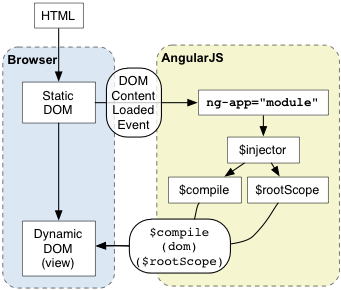
\includegraphics[width=10cm,keepaspectratio]{figures/concepts-startup.png}
%%\caption{Dinamikus kliensoldali HTML AngularJS-ben}
%\label{fig:angularhtml}
%\end{figure}

A hagyományos weboldal esetében a böngészőben megjelenített HTML a szerver oldali alkalmazás által van létrehozva.  A single-page alkalmazás ebben az esetben úgy jön létre, hogy AJAX felhasználásával betöltés után töltődnek be újabb részei az oldalnak\cite{angularbook}. AngularJS esetében ez a művelet a kliens oldalra kerül így a szerver inkább egy adatforrás és statikus tartalom szolgáltatóvá válik. Így lazább csatolást érünk el a szerver és kliens oldal között esetleg párhuzamosítva a fejlesztést és növelve az újrafelhasználhatóságot\cite{AngularDocConcepts}.





\subsection{Direktívák}

Az AngularJS fordító segítségével ki lehet terjeszteni a HTML szintaxist új attribútum és elem típusokkal, ezeket hívják direktívának. 

\lstset{language=HTML}
\begin{lstlisting}[frame=single]  
<ul>
  <li ng-repeat="action in user.actions">
    {{action.description}}
  </li>
</ul>
\end{lstlisting}

Magas szintről nézve a direktívák megjelölik a DOM elemeket és ennek hatására az AngularJS fordító speciális viselkedéssel bővíti ki ezeket az elemeket. A DOM-ot csak direktívák segítségével lehet befolyásolni AngularJS-ben és ez a szeparáció segít a tesztelésben. 

Beépített direktívák vannak, példáúl \lstinline{ng-repeat}, \lstinline{ng-click}, \lstinline{ng-show}, és ezek kiterjeszthetőek saját direktívákkal. Ekkor meg lehet határozni egy HTML templatet a direktívának, ami helyettesíti a DOM-ban a létező elemet az új template-tel és a direktíva \lstinline{link} attribútuma egy olyan függvény ami beállítja fordításkor a kiterjesztett viselkedést példáúl egy jQuery dátumkiválasztót kapcsol a DOM elemhez és ennek eseményeit hozzáköti a modellhez.


\subsection{Model-View-Controller}

Az MVC architektúra a desktop alkalmazások világában lett népszerű és csak az utóbbi években terjedt a webes alkalmazások világába. Az alap ötlet a tiszta elválasztása az adat kezelésnek (modell), az üzleti logikának (kontroller) és a megjelenítésnek (nézet). AngularJS alkalmazásokban a nézet a Document Object Model, a kontrollerek Javascript objektumok vagy függvények, és további objektum attribútumokban van tárolva a model.   

\subsubsection{Adatkötés}

jQuery és hasonló megoldások segítségével újratöltés nélkül frissíteni tudjuk a DOM-ot felhasználói események hatására vagy adatok frissítése esetében, de még az egyszerű esetekben sem biztos hogy triviális a DOM és adatok összehangolása. Az AngularJS ezt két irányú adatkötéssel próbálja megoldani ráadásul deklaratívan. Egy egyszerű példa adatkötésre:

\lstset{language=HTML}
\begin{lstlisting}[frame=single]  
<div ng-controller="HelloController">
  <input ng-model="greeting.text"/>
  <p>{{greeting.text}}, World!</p>
</div>
\end{lstlisting}
Ekkor az input mező módosítása automatikusan a model-t is frissíti és ez a cimkét is frissíti alatta. Ehhez az alap funkcionalitáshoz nem is szükséges más kódot írni.


\subsubsection{Függőséginjektálás}

Függőséginjektálás egy szoftver tervezési minta amiben beégetett függőségek helyett kicserélhető komponenseket használunk amiket akár futás időben is cserélhetünk. 

Ez egység tesztelés esetében válik hasznossá, hiszen jobban lehet izolálni alkalmazás logikát azzal, hogy függőségeket kicserélünk a tesztekben egy úgynevezett ``mocked'' függőséggel. Egy jó példa olyan függőségre amit teszt esetekben ki szeretnénk cserélni egy olyan kódrészlet ami egy különálló rendszernek az API-ját használja ráadásul állapotmódosítással járuló módon, amikor ezt ``mock-oljuk'', akkor tesztelni tudjuk az API felhasználását az API meghívása nélkül.

Egy kontroller a DOM -- vagy a nézet -- egy bizonyos részéhez van kötve, és függőséginjektálás során egy úgynevezett scope kontextus objektumhoz fér hozzá amin keresztül a modellhez férünk hozzá. Ez az elválasztás segít az újrafelhasználásban és karbantarthatóságban, mert, minden kontroller csak azt lát amit kell, hogy lásson és nem ``szennyezzük'' a globális környezetet. 

A scope objektumok egy hierarchiába vannak rendezve, létezik egy gyökér scope, és egymásbaágyazott kontrollerek scope objektumai prototípus örökléssel származnak egymásból.  
 
\begin{lstlisting}
function HelloController($scope) {
    $scope.greeting = {text: "Hello"}
}
\end{lstlisting}

\subsection{Szolgáltatások}

Az AngularJS szolgáltatások egyke példányok, amik bizonyos funkciót valósítanak meg az alkalmazásban, példáúl a \lstinline{http} szolgáltatás egy csomagoló a böngésző XMLHttpRequest objektuma körül és vele lehet AJAX hívásokat végrehajtani. 

AngularJS szolgáltatásokat injektálni kell, mint minden más függőséget, egy komponensbe, példáúl tudunk injektálni kontrollerbe, direktívába, szolgáltatásba stb. Természetesen saját szolgáltatást is lehet fejleszteni és ajánlott is az újrafelhasználandó logikát egy ilyen szolgáltatásba helyezni.

A kontrollerekbe mindig injektálni kell a \lstinline{scope} szolgáltatást, így megvalósul a kapcsolat a modell és a kontroller között.


%----------------------------------------------------------------------------
\section{MongoDB}
%----------------------------------------------------------------------------

A MongoDB egy nyílt forráskódú dokumentum-orientált adatbázis rendszer. A MongoDB nem egy relációs adatbázis, nem lehet SQL nyelv segítségével lekérdezéseket futtatni, nem támogat JOIN műveletet. A MongoDB BSON\footnote{Binary JSON} formátumban tárol kulcs-érték párokat. Az RDBMS\footnote{Relational Database Management System} alapfogalmai: adatbázis, tábla, sor, oszlop; a MongoDB megfelelői: adatbázis, kollekció, dokumentum, mező. Egy mező értéke lehet egszerű típus, lista vagy beágyazott dokumentum. A dokumentumok nem támogatnak sémát, tehát azonos fajta információnak lehet eltérő sémájú tartalma. 


\subsection{Indexelés}

MongoDB egy relációs adatbázishoz hasonlóan támogat indexelést, erre egy példa az~\ref{sec:dbprof} fejezetben lesz bemutatva. Érdekes fogalom a ``compound'' vagyis összetett index, ennek segítségével több mezőre is lehet egyszerre indexet építtetni és egy olyan lekérdezés ami egy termék gyártója és típusa alapján szűkít hatékony tud lenni.

Egy másik érdekes index fajta a ``multikey'' index, ami lehetővé teszi, hogy egy tömb értékű mező elemeit is indexeljük. Ha egy blogbejegyzés rekordban a bejegyzést kedvelő felhasználók tömbje van, akkor indexek támogatásával tudunk hatékony lekérdezéseket futtatni, példáúl szűrni az olyan bejegyzéseket, amiket Laci kedvelt.

\subsection{Replikáció}

A MongoDB egyik előnye, hogy nagyon könnyű benne adatbázisreplikációt megvalósítani. Egy replika halmaz több adatbázist tartalmaz aminek az egyik tagja a fő adatbázis ami elfogad írás műveleteket és a többi tag megkap minden változást és csak olvasás műveletet lehet rajtuk végrehajtani. A fő csomópont kiesése esetében a többi csomópont megszavaz egymás közül egy csomópontot aki átvegye a fő csomópont szerepét. Amikor a régi csomópont feléled, akkor szinkronizálja a változásokat és újra átveszi régi szerepét.

Az a kényelmes, hogy a kapcsolódó adatbázismeghajtók automatikusan kiválasztják a legközelebbi csomópontot az olvasáshoz. A közelség itt nem földrajzilag értendő, hanem a hálózati késleltetésre vonatkozik, sokszor összefügg a kettő. A csomópont szavazások és új szerepek kiosztásával nem kell foglalkoznia a fejlesztő aki kapcsolódik egy replika halmazhoz. 

\subsection{Sharding}

Egy nagyon sok adattal dolgozó rendszer túlterhelhet egy MongoDB adatbázist és ezt lehet egy darabig függőleges skálázással orvosolni, vagyis több fizikai erőforrást biztosítunk az adatbázisnak, de a terhelés állandó növekedése mellett csak időt nyerünk vele. 

Ehelyett a MongoDB vízszintes skálázhatóságot tesz lehetővé ``sharding'' segítségével. Ekkor az adatok partícionálása történik meg, a különböző partíciók különböző adatbázisokból lesznek elérhetőek. Az adatok partícionálása egy rögzített mező mentén történik, ezt később nem lehet megváltoztatni. Példáúl egy dokumentumszerkesztő rendszerben érdemes partícionálni a dokumentum tulajdonosa mentén, ekkor egy adatbázisra nézve csökken az írási és olvasási műveletek átlagszáma, ha egy felhasználó munkafolyamatot indít akkor csak az egyik adatbázis partícióban fog dolgozni.

A partícionáló rendszer próbál egyensúlyozottan partícionálni és, ha az egyik partíció megnő a többihez képest, akkor átlátszó módon átmozgat rekordokat egy másik partícióba.

A sharding és a replikáció egyszerre használható és kombinálható, példáúl három partíciónk lehet és mind a háromban három-három replika halmazunk lehet, így összesen kilenc csomópontunk lesz.



\subsection{ACID}

Fontos megjegyezni, hogy a RDBMS rendszerekkel szemben a MongoDB nem tud ACID trazakciókat biztosítani \cite{acidref}. 
\begin{enumerate}
\item{Atomicitás}: csak dokumentum szintű atomikus műveletek biztosítottak, ha több kollekció vagy dokumentumon átívelő atomikus tranzakciókat szeretnénk, akkor vagy használjunk RDBMS-t, vagy saját magunk kell egy zárolási mechanizmust fejleszteni.
\item{Konzisztencia}: replikáció esetében a fő adatbázis csomópontot érintik az írás műveletek, az olvasás műveletek meg -- opcionálisan --  a ``közelebb'' tartózkodó csomóponthoz fordulnak. Ebben az esetben ``eventual consistency''-ről beszélünk és nem biztosított, hogy friss adatot olvasunk.  
\item{Izoláció}: MongoDB esetében nem lehet beszélni izolációról, mert csak dokumentumszintű tranzakciók vannak és minden dokumentum művelet hatása azonnal elérhető a többi folyamat számára. 
\item{Tartósság}: teljesítmény árán lehet a tartósságot növelni, példáúl úgy, hogy egy írás művelet a többi csomópontra is íródjon mielőtt visszatérne.
\end{enumerate}

%A CAP\footnote{(C)onsistency - Konzisztencia, (A)vailability - Elérhetőség, (P)artition tolerance - Partícionálás tolerancia} tétel kijelenti, hogy egy elosztott rendszer nem tudja egyszerre teljesíteni a ...

A 32 bites rendszereken a mongoDB szerver csak 2GB tárral gazdálkodhat, ugyanakkor a 64 bites esetben csak a hardver mérete korlátozza.










%----------------------------------------------------------------------------
\section{Node.JS}
%----------------------------------------------------------------------------

Node.js egy Javascript alapú platform amivel skálázható szerveroldali alkalmazásokat hoznak létre és a Google V8 Javascript motorra épül. Node.js egy webszerver modult is tartalmaz aminek segítségével önmaga is tud webszerverként működni. A platform alapítója azzal a céllal hozta létre a Node.js-t hogy egyszerűen lehessen olyan weboldalakat létrehozni amik képesek kétirányú kommunikációra és én is ezért választottam mint szerver oldali technológia ugyanis a legkönnyebben integrálódik a Socket.IO rendszerrel.  Egy másik ok az, hogy nagyon könnyen lehet benne prototipizálni.



\subsection{Nem-blokkoló IO}

A legfeltűnőbb sajátossága a Node.JS platformnak az, hogy majdnem semmilyen hívás nem blokkoló és elsőre elég furcsa csupa aszinkron függvényekkel dolgozni. Ebben rejlik a Node.JS skálázhatósága, ahelyett hogy szálakat allokáljon HTTP kérésekhez, amik drágák és nem lehet belőlük nagyon sok, aszinkron módon az operációs rendszertől vár értesítést, hogy van egy bejövő kérés és addig alszik. A Nem-blokkoló IO abban segít, hogy sohasem vár egy erőforrásra, hanem , példáúl, adatbázis lekérdezést indít, kiszolgál néhány más kérést és később megérkezik az adatbázistól a kért adat. 

Ennek egy következménye az úgynevezett ``shared-state concurrency'' amiben a különböző kérések kiszolgálása nem külön folyamat vagy szálban fut, így egy memóriabeli változó megváltozhat a hívás és a callback lefutása között egy másik kérés által. Erre tipikus ellenpélda az Apache szerver ami minden kérésre új szálat indít friss állapottal. Mivel egy folyamatban fut a Node szerver, lehetséges blokkolni a szervert példáúl azzal, hogy egy callback-ben nagy számot faktorizálunk. Node valójában nem valósít meg konkurrenciát hiszen egyszerre csak egy függvény fut, de mivel ezek gyorsan futnak V8 alatt és nem blokkolnak ezért hatékonyan tud átlagos hardveren több ezer lekérdezést kiszolgálni másodpercenként\cite{nodebook}.

\subsection{Modulkezelés}

A böngésző világában egy külső Javascript könyvtár használatánál -- példáúl a gyakori \lstinline|<script src='http://code. jquery.com/jquery-1.6.0.js'>| -- valószínű, hogy a globális névtérbe kerülnek az új deklarált változók. A jQuery a ``\$'' változót deklarálja a globális névtérben, és ha beteszünk egy másik modult ami ugyanezt csinálja, akkor az első nem fog már működni. 


A szerveroldali Javascript világában az npm\footnote{Node Packaged Modules} segítségével kell 3rd party modulokat telepíteni és egyidejűleg izolált környezetet biztosítani a különböző projekteknek. A Python világában a virtualenv az eszköz amivel lehet izolált környezetet biztosítani és mellette a pip parancs segítségével lehet modulokat telepíteni. Virtualenv-vel szemben az npm alapértelmezetten a lokális környezetünkbe telepít modulokat, virtualenv esetében ez fordítva van, ez néha zavaró, ha a fejlesztő elfelejti aktiválni a környezetet és rossz környezetbe települ a csomag.
Az npm továbbá abban is segít, hogy egy telepített függőséget lehetséges egyből bele is íratni a függőségleíróba:
\lstset{language=bash}   
\lstinline{npm install --save express}.
Ez a függőség leíró a package.json fájl és \lstinline{npm install} paranccsal (paraméter nélkül) minden függőség települ. Ez nem csak a rendezettség miatt fontos, hanem amiatt is, hogy sok node webhosting megoldás -- többek között az általam használt nodejitsu\footnote{http://www.nodejitsu.com} -- a package.json csomagjait telepíti az alkalmazásunkhoz.   

A csomagok a require modul segítségével töltődnek be dinamikusan, példáúl
\begin{lstlisting}
var fs = require('fs');
\end{lstlisting}





%----------------------------------------------------------------------------
\section{MEAN stack}
%----------------------------------------------------------------------------

%http://blog.mongodb.org/post/49262866911/the-mean-stack-mongodb-expressjs-angularjs-and

A MEAN, a MongoDB, Express.JS, Angular.JS, Node.JS technológiáknak a rövidítése, és a lényege az, hogy adatbázisban, szerver oldalon és kliens oldalon végig JSON objektumokkal dolgozunk ráadásul nincs is szükség még más keretrendszerre weblapok készítéséhez, ez egy úgynevezett ``full-stack'' megoldás. A MEAN előnye az, hogy a kölönböző rétegekre specializált fejlesztők akik egy ilyen fejlesztésen dolgoznak könnyebben megértik a többi réteg kódját, hiszen Javascript nyelven történik mindhárom fejlesztés. 


\section{Felhasznált fejlesztői eszközök}

Ebben a fejezetben azokat a fejleszői és dokumentáló eszközöket mutatom be röviden amikez szakdolgozatomhoz felhasználtam.

\subsection{Jetbrains Webstorm}

A Javascript kódot Jetbrains Webstorm fejlesztőkörnyezetben szerkesztettem. A fő okok amiért ezt választottam:
\begin{itemize}
\item bizonyos mértékben támogat ``IntelliSense'' jellegű kódkiegészítést és kódvalidálást, ami szkriptnyelvek esetében elég hasznos,
\item lehet vele debuggolni egy NodeJS szerveralkalmazást,
\item támogat kódnavigálást.

\end{itemize}

\begin{figure}[!ht]
\centering
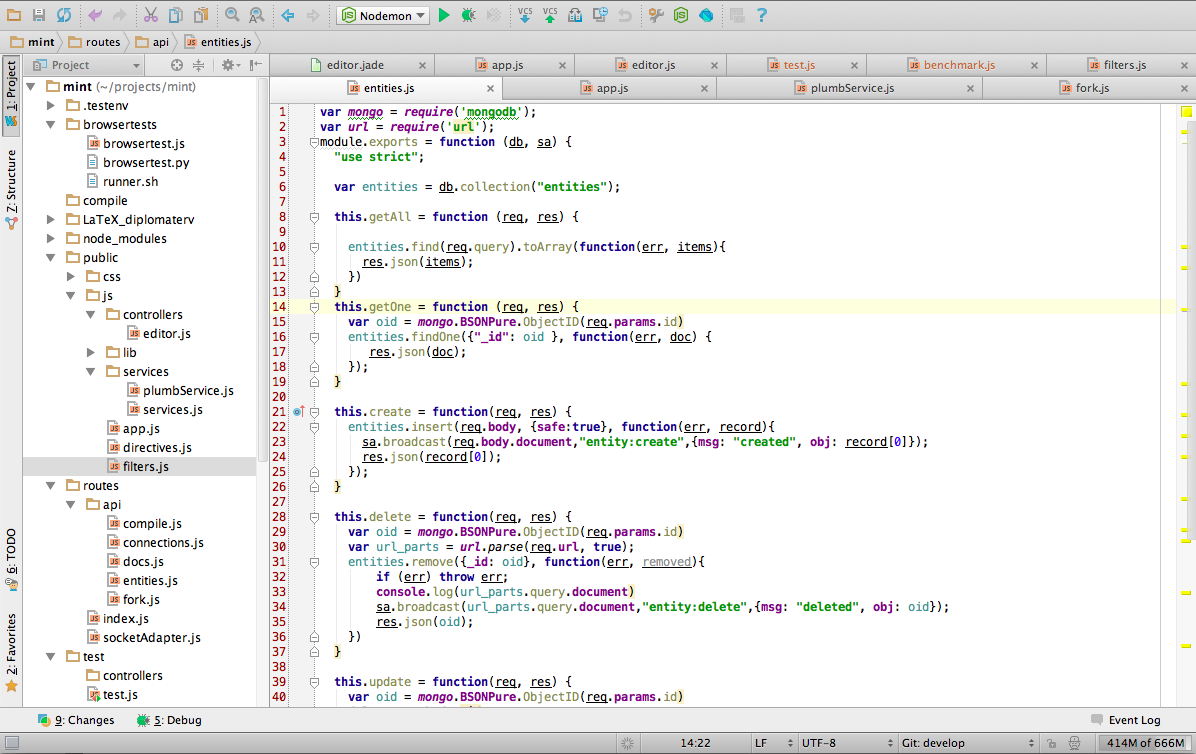
\includegraphics[width=15cm,keepaspectratio]{figures/webstorm.png}
\caption{Jetbrains Webstorm}
\label{fig:webstorm}
\end{figure}

\subsection{Chrome Developer Toolbar}

Az alkalmazásomat fejlesztés közben Google Chrome-ban próbáltam ki főleg a fejlesztői panel miatt, amivel beállítva egy breakpointot vagy a \lstinline{debugger} sor beszúrásával hatékonyan lehet debuggolni. Ráadásul a breakpointnál megállva a Javascript shell az aktuális kontextusban működik és lehet azt a kontextust manipulálni parancsok beírásával.


\subsection{Node Inspector}

A Node Inspector eszköz, ami \url{https://github.com/node-inspector/node-inspector} címről szerezhető meg egy olyan szerveralkalmazás amivel egy Chrome Developer Toolbar példányt a NodeJS szerveroldali alkalmazásra lehet csatolni és ugyanazt a debuggolási funkcionalitást lehet elérni szerveroldalon mint kliensoldalon. Sokszor kényelmesebb volt ezt használni a Webstorm debuggernél.

\subsection{Wireshark}

A Wireshark protokollanalizátor a Websockets forgalom vizsgálatára volt hasznos amit a~\ref{sec:simprof} fejezetben részletezek.

\subsection{Lucidcharts}

A rendszerábrákhoz Lucidcharts szerkesztőt használtam, mert hatékonyan lehet benne jó minőségű ábrákat gyártani.

\subsection{Latex}

A jelen szöveges dokumentumot Latex-ben írtam a diplomaterv portál sablonját felhasználva. Elég sok időbe került amire mindent beállítottam, de a következő okok miatt találtam nagyon hatékony eszköznek:

\begin{itemize}
\item A dokumentumot fel lehet darabolni több fájlba, akár több mélységben is, majd a fordító összefésüli,
\item nem valószínű, hogy lokális módosítások elrontják a dokumentum egy másik részét,
\item az ábrák egy helyre vannak gyűjtve, ki tudok cserélni egy ábrát úgy, hogy ne kelljen megnyitanom a szerkesztőt,
\item kevésbé valószínű, hogy a Notepad jellegű szövegszerkesztőm lefagy, mint az, hogy egy bonyolultabb szövegszerkesztő lefagyjon,
\item könnyebbnek találtam az ábrák beszúrását és testreszabását.
\end{itemize}

Sokszor nehéz debuggolni, hogy miért nem fordul le a dokumentum.

\subsection{Git}

Fontos volt, hogy a munkám ne vesszen el, így egy Git repository-ba helyeztem el, amit egy szerverre szinkronizáltam rendszeresen. A szöveges dokumentumot is beletettem a repository-ba, így a teljes munkám előző állapotait is tudtam böngészni.



